\section{Arquitetura}

\subsection{Definição da Arquitetura}

A arquitetura proposta para o sistema web da loja \textbf{Tropical Mix} baseia-se em um modelo multicamadas, que separa claramente a interface de apresentação (\textit{front-end}), a lógica de negócio (\textit{back-end}) e o armazenamento de dados (banco de dados). Essa abordagem visa garantir modularidade, escalabilidade e facilidade de manutenção, além de permitir futuras expansões do sistema.

No nível de apresentação, o \textit{front-end} foi desenvolvido utilizando a biblioteca \textbf{React}, em conjunto com \textbf{JavaScript} e \textbf{HTML/CSS}. Essa combinação possibilita a criação de uma interface moderna, interativa e responsiva, permitindo que o sistema seja acessado por diversas pessoas.

Na camada de aplicação, responsável pela lógica de negócio, foi adotada a linguagem \textbf{Python} juntamente com o framework \textbf{Flask}. Essa tecnologia foi escolhida por oferecer leveza, flexibilidade e facilidade de integração com outras ferramentas, além de possuir uma ampla comunidade de suporte.

Para o gerenciamento e persistência de dados, o sistema utiliza o \textbf{MySQL} como banco de dados relacional. Essa escolha se deve à sua robustez, confiabilidade e compatibilidade com aplicações web modernas.

Além disso, a comunicação entre o \textit{front-end} e o \textit{back-end} é realizada via \textbf{API REST}, utilizando o formato \textbf{JSON} para o envio e recebimento de dados. Essa arquitetura baseada em serviços favorece a escalabilidade do sistema, permitindo que novas funcionalidades ou módulos possam ser integrados sem comprometer a estrutura existente.

\subsection{Diagrama da Arquitetura}

A Figura~\ref{fig:arquitetura} apresenta o diagrama de implantação do sistema, ilustrando a interação entre as camadas e os principais componentes que compõem a aplicação web.

\begin{figure}[H]
    \centering
    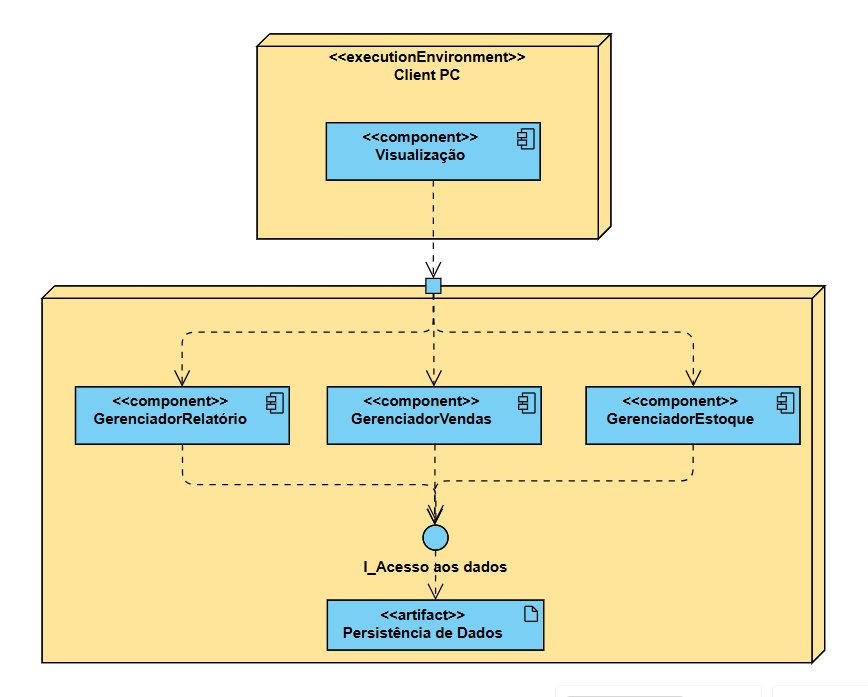
\includegraphics[width=0.9\textwidth]{LaTex/Capítulos/img/Desenvolvimento do Projeto/Arquitetura/arquitetura.png}
    \caption{Diagrama de Implantação}
    \fonte{Elaborado pelos autores.}
    \label{fig:arquitetura}
\end{figure}

Opcionalmente, a Figura~\ref{fig:componentes} apresenta o diagrama de componentes, que detalha a estrutura lógica do sistema e as dependências entre os módulos internos.

\begin{figure}[H]
  \centering
  \includegraphics[width=0.9\textwidth]{LaTex/Capítulos/img/Desenvolvimento do Projeto/Arquitetura/Diagrama_componentes.png}
  \caption{Diagrama de Componentes.}
  \fonte{Elaborado pelos autores.}
  \label{fig:componentes}
\end{figure}




